\documentclass[a4paper,twoside]{article}

\usepackage{RR}
\usepackage{hyperref}
%\usepackage[frenchb]{babel}
%\usepackage[T1]{fontenc} % avec T1 comme option  d'encodage c'est ben mieux, surtout pour taper du français.
\usepackage[utf8]{inputenc}
\usepackage[table]{xcolor}
\usepackage{color}
\usepackage{graphicx}
\usepackage{amsmath, amsthm}
\usepackage{stmaryrd}
\usepackage{lscape}

\usepackage{url} \urlstyle{sf}%
\usepackage{graphicx}%
\usepackage{subfigure}
\usepackage{listings}%

\lstset{%
  basicstyle=\scriptsize,%
  numbers=left,
  %columns=fullflexible,%
  language=XML,%
  %frame=shadowbox,
    frame=lbtr,%
  frameround=tttt,%
  tabsize=2,
  breaklines=true
}%
\usepackage{tikz}
\usetikzlibrary{decorations.pathreplacing,positioning}
\usepackage{array}
\usepackage{xspace}

\newcommand{\ie}[0]{{\em i.e.},\xspace}
\newcommand{\vs}[0]{{\em vs.}\xspace}
\newcommand{\eg}[0]{{\em e.g.},\xspace}
\newcommand{\etal}[0]{{\em et al.}\xspace}
\newcommand{\wrt}[0]{{\em w.r.t.}\xspace}
\newcommand{\aka}[0]{{\em a.k.a.}\xspace}

\sloppy

%%% FORMAT DOCUMENT

\def\textfraction{0}
\def\floatpagefraction{1}
\def\topnumber{3}
\def\bottomnumber{3}
\def\totalnumber{3}
\def\topfraction{1}
\def\bottomfraction{1}

%%.
\usepackage{bold-extra,graphicx,latexsym,mathrsfs,subfigure,xspace}

\usepackage{color}
\usepackage{array}
\usepackage{longtable}
\usepackage{calc}
\usepackage{multirow}
\usepackage{hhline}
\usepackage{ifthen}

\usepackage{hyperref}

\newcolumntype{M}[1]{>{\raggedleft}m{#1}}
\newcommand{\discovery}{DISCOVERY\xspace}

%% CT %%
\newcommand{\ftodo}[2][\relax]  % \TODO[editor]{text} 
  {\ensuremath{{}^{\mbox{\tiny\bf #1}}}~\textbf{#2}}

\begin{document}

\RRNo{XXXX}
\RRdate{April 2016}

\RRprojet{DISCOVERY IPL}

% \author{Adrien L?bre\inst{1,3} \and Jonathan Pastor\inst{1,3} \and Marin Bertier \inst{2,3} \and Fr?d?ric Desprez\inst{3} \and Jonathan Rouzaud-Cornabas\inst{3} \and C?dric Tedeschi \inst{3,4}\and Paolo Anedda\inst{5} \and Gianluigi Zanetti\inst{5} 
% \and Ramon Nou\inst{6} \and Toni Cortes\inst{6} \and Etienne Riviere\inst{7} \and Thomas Ropars\inst{8}}
% \institute{LINA / Mines Nantes, France 
% \and IRISA / INSA de Rennes, France
% \and INRIA, France
% \and IRISA / Universit? de Rennes 1, France
% \and Center for Advanced Studies, Research and Development in Sardinia (CRS4), Italy
% \and Barcelona Supercomputing Center (BSC), Spain
% \and Universit? de Neuch?tel (UniNe), Switzerland
% \and Ecole Polytechnique F?d?rale de Lausanne (EPFL), Switzerland} 

%
% Title and Authors
%
\RRauthor{
A. Lebre\thanks[Inria]{Inria, France, Email: \url{FirstName.LastName@inria.fr}}\thanks[EMN]{Mines Nantes/LINA (UMR 6241), France.}%\inst{1} 
\and 
J. Pastor\thanksref{Inria}\thanksref{EMN} 
\and 
Frederic Desprez\thanksref{Inria}  
}

\authorhead{A. Lebre et al.}

\RRtitle{Révisiter les mécanismes internes du système OpenStack en vue d'opérer des infrastructures de type nuage massivement distribuées}
\RRetitle{
A Ring to Rule Them All - Revising OpenStack Internals to Operate Massively Distributed Clouds}%\thanks{This report ....}}
\titlehead{The DISCOVERY Initiative}

%\RRnote {XXXX}

\RRkeyword{Fog, Edge Computing, 
Peer To Peer,
Self-*,
Sustainability,
Efficiency,
OpenStack, 
Future Internet.
}

\RRmotcle{Calcul utilitaire basé sur la localité, systèmes pair-à-pair, self-*, durabilité,OpenStack 
Internet du futur}

%
% Abstract
%
\RRabstract{

  {\small 

The deployment of micro/nano data-centers in network point of presence offers an opportunity to deliver a more sustainable and efficient infrastructure for Cloud Computing. Among the different challenges we need to address to favor the adoption of such a model, the development of a system in charge of turning such a complex and diverse network of resources into a collection of abstracted computing facilities that are convenient to administrate and use is critical.

In this report, we introduce the premises of such a system. The novelty of our work is that instead of developing a system from scratch, we revised the OpenStack solution in order to operate such an infrastructure in a distributed manner leveraging P2P mechanisms. More precisely, we describe how we revised the Nova service by leveraging a distributed key/value store instead of the centralized SQL backend. We present experiments that validated the correct behavior of our prototype, while having promising performance using several clusters composed of servers of the Grid'5000 testbed. We believe that such a strategy is promising and paves the way to a first large-scale and WAN-wide IaaS manager.

}
}

\RRresume{

  {\small 

La tendance actuelle pour supporter la demande croissante d'informatique
utilitaire consiste à construire des centres de données de plus en plus grands,
dans un nombre limité de lieux stratégiques. Cette approche permet sans aucun
doute de satisfaire la demande actuelle tout en conservant une approche
centralisée de la gestion de ces ressources, mais elle reste loin de pouvoir
fournir des infrastructures répondant aux contraintes actuelles et futures en
termes d’efficacité, de juridiction ou encore de durabilité.  L’objectif de
l'initiative DISCOVERY\footnote{\url{http://beyondtheclouds.github.io}} est de
concevoir le \emph{LUC OS},  un système de gestion distribuée des ressources qui permettra de
tirer parti de n’importe quel n\oe ud réseau constituant la dorsale d’Internet
afin de fournir une nouvelle génération d’informatique utilitaire, plus apte à
prendre en compte la dispersion géographique des utilisateurs et leur demande
toujours croissante. 

Après avoir rappelé les objectifs de l'initiative DISCOVERY et expliqué
pourquoi les approches type fédération ne sont pas adaptées pour opérer une
infrastructure d'informatique utilitaire intégrée au réseau, nous présentons les
prémisses de notre système.  Nous expliquerons notamment pourquoi et comment
nous avons choisi de démarrer des travaux visant à revisiter la conception de
la solution Openstack. De notre point de vue, choisir d'appuyer nos travaux sur
cette solution est une stratégie judicieuse à la vue de la complexité des
systèmes de gestion des plateformes IaaS et de la vélocité des solutions
open-source. 
}
}

\URRennes
\makeRR

%%%

\section{Introduction}

\subsection{Massively distributed cloud}

\begin{itemize}

	\item A massively distributed cloud targets management of thousand of hosts around a wide territory.	
	
	\item This scale order is currently reached by file sharing systems like bittorrent.

	\item At this scale, failure becomes the norm.

	\item Recent works propose to leverage on peer to peer overlay.

	\item Some peer to peer overlays can take advantage of locality. It enables to build systems that can take
		  into account network bandwidth and latency.

	\item We propose to leverage on locality based peer to peer mechanisms to reach an high scalability IaaS.

\end{itemize}

\subsection{Toolkit for IaaS}

\begin{itemize}

	\item A toolkit is a building block that can be used for the construction of systems.

	\item The objective of a toolkit is to provide "state of the art" solutions to known problems. It enables the
		  focus on "Top level" works.

	\item It provides a set of components, which once assembled constitute an operational system.

	\item Recent studies of "state of art IaaS systems" (Openstack, Cloudstack, OpenNebula, ...) showed that they
		  were constructed over same concepts. It enables the design of IaaS toolkit.

	\item The massively distributed IaaS toolkit will provides "state of the arts" mechanism to solve both scalability and locality points.

	\item The toolkit will have to integrate well on existing systems: we propose to leverage Openstack project.

\end{itemize}


\section{Revising OpenStack}
\label{sec:leveraging-openstack}

OpenStack is an open-source project that aims at developing a complete cloud management
system. Similary to the reference architecture described in the previous Section, it is
composed of several services, each one dealing with a particular
aspect of a Cloud infrastructure as depicted in Figure~\ref{fig:openstack}.

\begin{figure}[htbp]
        \centering
        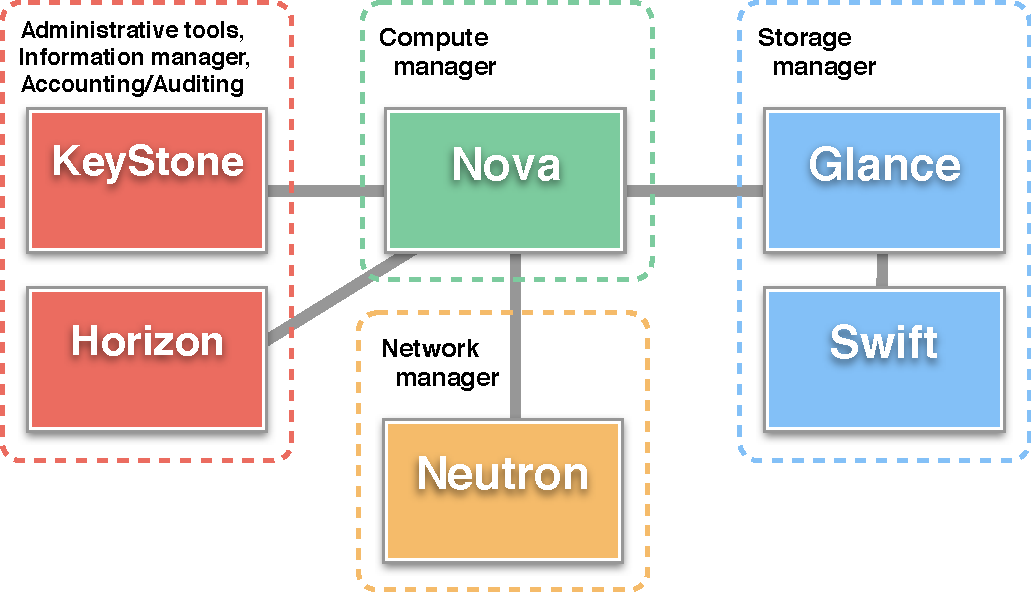
\includegraphics[width=6cm]{figures/OpenStack_architecture.pdf}
\vspace*{-.3cm}
        \caption{Services composing OpenStack.}
        \label{fig:openstack}
\vspace*{-.3cm}
\end{figure}


OpenStack relies on two kinds
of nodes: controller and compute node. The former is in charge of managing and
distributing work to the latter that provides computing/storage resources to end-users. In
other words, the controllers correspond to the different services introduced in the
previous section while the compute nodes host the VMs.

From the software point of view, the OpenStack architecture is based on the ``shared
nothing" principles: each controller (\ie each service) is connected to the others via two
different way:

\begin{itemize}
   \setlength{\itemsep}{0pt}
  \setlength{\parskip}{0pt}
   \setlength{\parsep}{0pt}
\item \textbf{A messaging queue} that enables the collaboration between sub-services of a
  controller.
\item \textbf{A SQL database} (DB) that stores inner states of a controller.
\end{itemize}

Finally, the controllers interact with each other through REST APIs or directly by accessing
the inner-state that are stored in the differents DBs.
%\AL[JP]{Is it correct ? How the controllers interaact/collabore ?}

Considering the current structure of OpenStack, the main limitation to make it distributed
is related to the SQL databases. Indeed, while OpenStack relies on the
RabbitMQ messaging service, which is articulated around a centralized
broker, there are few implementations of  P2P messaging
service such as ActiveMQ~\cite{activemq:2011} or ZeroMQ~\cite{zeromq:2013} that would be adapted to the LUC requirements.
% \section{Towards a fully distributed OpenStack deployment}
%
% The discovery initiative targets the delivery of an utility computing platform
% that will be working on top of existing network backbone facilities. Starting
% the development of such a platform from zero would require a titanic effort: in
% order to spare a giant development time, the Discovery initiative proposes to
% leverage the OpenStack project: this will serve as the foundation of the
% LUC-OS.
%
% In order to structure the LUC-OS on a fully distributed peer to peer
% functionning, OpenStack would be required to be fault tolerant and to be able to
% fit on a multi-site configuration. In the current situation, it requires some
% adaptations: in this section we propose some modifications that
% have been introduced in the Nova controller, to meet the two
% aforementioned criterions.
%
% \subsection{Replacing the relational backend by a Key/value store}
%
% From today's perspective, most of the OpenStack deployment are involving few
% nodes, thus not requiring more thant one controller. However, to meet the fault
% tolerance criterion, one needs to use \textit{High availibility} deployment by
% combining two components \textit{HAProxy} (load balancing) with
% \textit{Galera} (Relational database replication).
The first way to bypass the MySQL limitation is to
% a controller between distinct locations,
%\ie to be able to scale in/out the services it offers, is to
deploy each controller DB on each location and to synchronize the different DB
instances with a dedicated mechanism~\cite{kemme:vldb2010}. By such a mean, when a
controller processes a request and performs some actions on one site, changes in the
inner-state are also propagated to all the other locations. From a certain point of view,
it gives the illusion that there is only one DB for each service. Although the technique
described has been used in different proof-of-concepts, current DB synchronization
mechanisms are not scalable enough to cope with a LUC infrastructure deployed on large
number of geographical sites.

Another approach is to replace the DBs used in OpenStack by a more suitable storage
backend that would provide a better scalability. Distributed Hash Tables (DHTs) and more
recently key/value systems built on top of the DHT concept such as
\emph{Dynamo}~\cite{decandia:dynamo} have demonstrated their efficiency in terms of
scalability and fault tolerance properties.
%
In light of this, we have revisited the Nova controller, \ie the VM manager of OpenStack,
in order to to replace the current MySQL DB system by \textit{REDIS} ~\cite{han:2011},
a \textit{key/value store}.
% that extends the principles followed by the \textit{Dynamo}. %with more advanced storage and query features.
Technically speaking, we modified the Nova database driver. Indeed, the  Nova software architecture has been
organised in a way which ensures that each of its sub-services does not directly manipulate the database: they have an indirect
access through a service called ``nova-conductor" which in turn works with an
implementation of the \textbf{"nova.db.api"} programming interface. Developers of Nova
provide an implementation of this interface that is using \textit{SQLAlchemy} to
manipulate a relational database. We developed a second implementation of this interface
that replaces every call to the \textit{SQLAlchemy} by a call to a
custom key/value store
driver.  This enables  Nova's services to work with REDIS by only changing the
database driver, limiting the level of intrusiveness in the original source code.
Thanks to this modification, it is possible to instanciate  a distributed
cloud and operate it through a single instance of OpenStack composed
of several Nova controllers deployed on distinct sites.
Figure~\ref{fig:newnova} depictes such a deployment.
%
Each controller executes a REDIS instance that is configured to work in
a clustering way with other instances.
One or several controllers can be deployed on each site according to
the expected demand in terms of end-users. Finally, a controller can be
deployed either on a dedicated node or be mutalized with a compute
one as illustrated for Site 3. We higlight that any controller can
provision VMs by orchestrating services on the whole infrastructure and not only on the site
where it is deployed. Such a behavior is possible thanks to the AMQP
bus and the key/value store that go through all controllers.
%
Finally, it is noteworthy that key/value stores that
focus on high-availability and partition tolerance criteria like
Cassandra~\cite{lakshman:2010} would be more appropriate than REDIS
for a production deployment. We chose REDIS for its usage simplicity.

\begin{figure}[htbp]
        \centering
\vspace*{-.4cm}        \hspace*{-.2cm}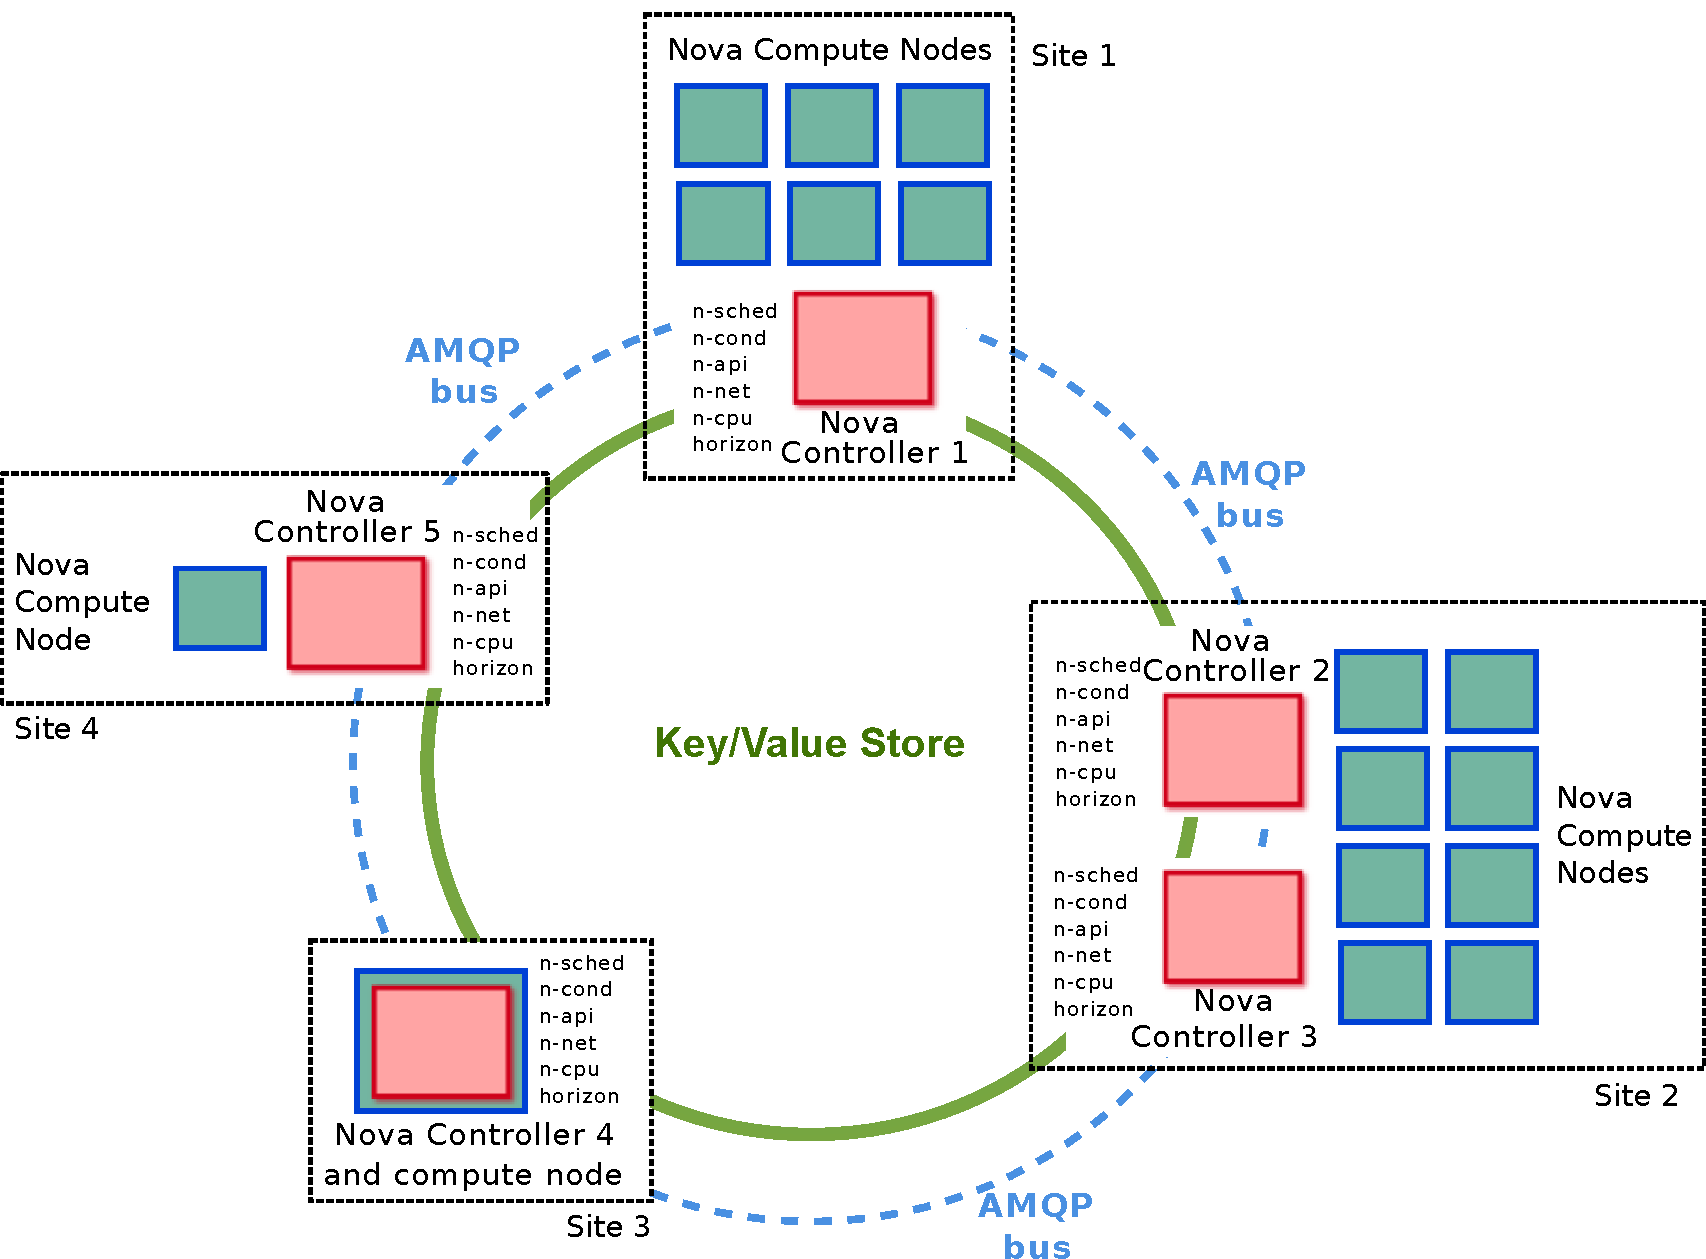
\includegraphics[width=.51\textwidth]{figures/OpenStack_distributed.pdf}
        \caption{Nova controllers are connected through a shared key/value backend
        and the AMQP bus.}
      \label{fig:newnova}
\vspace*{-.3cm}
\end{figure}

Our prototype is under evaluation.
However, preliminary experiments  have been performed throughout 4
sites of Grid'5000  including 12 compute nodes  and 4 controllers
overall. While this
infrastructure was rather small in comparison to our target, it aimed
at validating the interconnection of several controllers WANwide and
the correct behaviour of  OpenStack using our noSQL backend.
Our prototype suceeded to provision 500 VMs in 300 seconds
(each controller creating 125 VMs in parallel).
A second experiment validated the provisionning
of 2000 VMs in less than 30 min.  We are currently performing comparisons
between OpenStack using the historical MYSQL backend \textit{v.s.,}
using a key/value store backend. Our goal is to validate that
manipulating internal states of Openstack through
a noSQL deliver performances in the same order of the MySQL
ones.


\section{Experimental validation on Grid'5000}
\label{sec:eval}

The validation of our prototype has been performed thanks to the Grid'5000
testbed \cite{grid5000}. Grid'5000 is a large-scale and versatile experimental
testbed for experiment driven research in Computer Science, which enables
researchers to get an access to a large amount of computing resources
($\sim$ 1000 nodes spread over 10 sites). This delivery of computing resources
takes the form of bare-metal machines, on which fully customised software stacks
can deployed, thus giving a very fine control of the experimental conditions.

Various tools have been developed to provide an ease of use, such as monitoring
information about networking and power consumption or programming libraries to
fine tune each aspect composing an experiment. With this in mind, we developed
our prototype using the Execo framework \cite{imbert:hal-00861886} which helped
us to deploy and configure each node composing our chosen software stack (Ubuntu
14.04, a modified version of OpenStack "devstack", and the RIAK key/value store).

Our validation scenario has consisted in the creation of 30 VMs
through 10 different Nova controllers deployed on one cluster located
in Nantes. This experiment enabled us to confirm that OpenStack's
services were working correctly with the key/value store.
% that the relational backend
%used by the several components can be satisfactorily replaced by this
%new distributed key/value system.
Although further experiments are
required to test the scalability as well as the effect
of geographical distances on the reliability and efficiency, we are
confident about our approach as several distributed key/value stores
are already used WANWide.

% \AL[JP]{Finalize the text of this section, please be consistent the
%   announcement at the end of the introduction}
% Several test-cases with 10 nodes to evaluate
% the efficiency of the new framework:\begin{inparaenum}[1\upshape)]
% \item 1 site, 1 controller, 9 compute nodes
% \item 1 site, 10 controllesr, 0 compute node
% \item 2 sites, 1 controller/by site, 4 compute nodes/by site
% \item and 2 sites, 5 controllers/by site, 0 compute nodes/by site
% \end{inparaenum}



%test infrastructure is a tedious task if one has to do it
%manually. In order to simplify tests, we create a tool based on \texttt{Execo}
%\cite{imbert:hal-00861886} that: find a time slot when the resources
%are available on the several sites.
% deploy Ubuntu 14.04 on all the nodes, install RIAK DB and setup
% our modified version of devstack (with automatic node configuration), and
% finally start the distributed OpenStack infrastructure. The duration of the
% deployment is around 1 hour, depending on the cluster hardware and the
% total number of nodes. Finally, the tool provides some options that simplifies
% the management of the different test-cases, namely the number of sites,
% controller by site and compute nodes by site.

%\begin{figure}[h!]
%    \centering
%    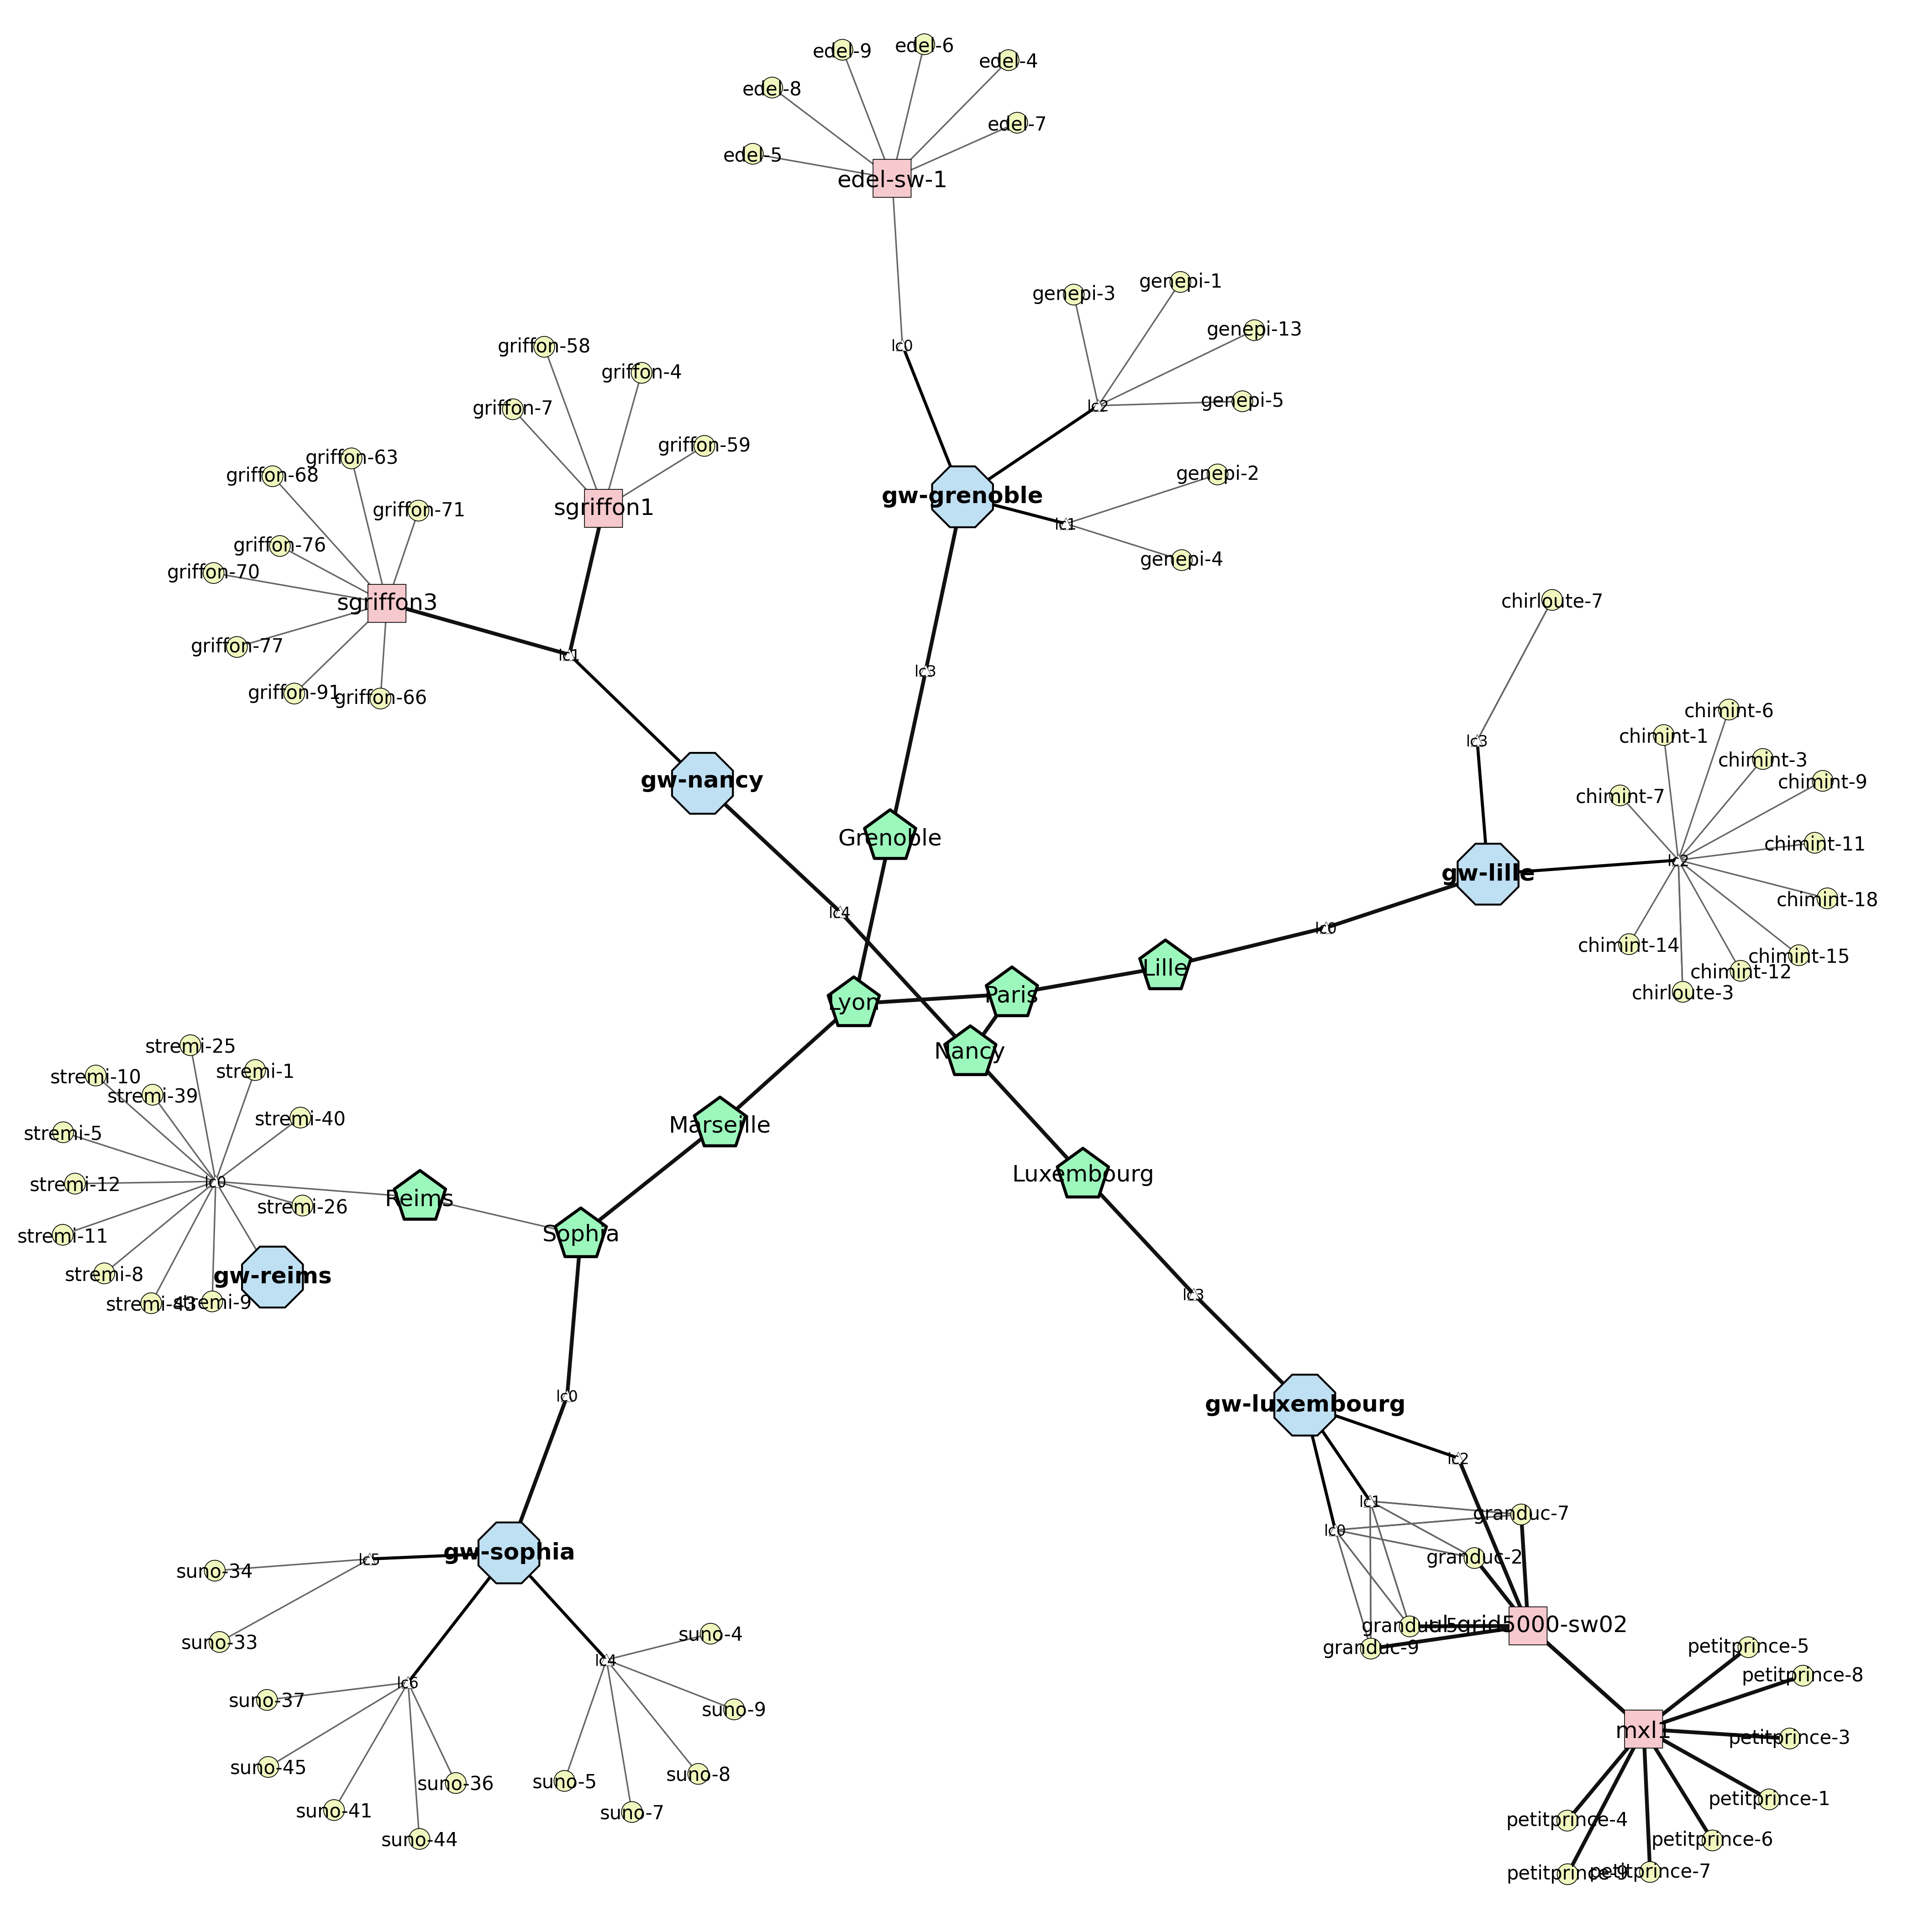
\includegraphics[width=7cm]{figures/6_sites.png}
%    \caption{Test-cases on the Grid'5000 platform involving 6
%    geographically-spreaded sites each hosting 2 controllers and 10 computes
%    nodes.}
%\end{figure}


%\subsubsection{Test-cases}
%\paragraph{Monosite}
%\paragraph{Multisite: 1 controller per site}
%\paragraph{Multisite: 10 controllers per site}

 


Cloud Computing has entered our everyday life at a very high speed and huge scale. From classic high performance computing simulations to the management of huge amounts of data coming from mobile devices and sensors, its impact can no longer be minimized. While a lot of progress has already been made in Cloud technologies, there are several concerns that limit the complete adoption of the Cloud Computing paradigm.

In a previous report~\cite{lebre:hal-00854204}, we outlined that, in addition to these concerns, the current model of UC is limited by intrinsic issues. Instead of following the current trend by trying to cope with existing platforms and network interfaces, we proposed to take a different direction by promoting the design of a system that will be efficient and sustainable at the same time, putting knowledge and intelligence directly into the network backbone itself. The innovative approach we introduced will definitely tackle and go beyond Cloud Computing limitations. Our objective is to pave the way for a new generation of Utility Computing that better matches the Internet structure by means of advanced operating mechanisms. By offering the possibility to tightly couple UC servers and network backbones throughout distinct sites and operate them remotely, the LUC OS technology may lead to major changes in the design of UC infrastructures as well as in their environmental impact. The internal mechanisms of the LUC OS should be topology dependent and resources efficient. The natural distribution of the nodes through the different points of presence should be an advantage, which allows to process a request according to its scale: Local requests should be computed locally, while large computations should benefit from a large number of nodes.

The first step toward this highly distributed Cloud infrastructure taking into account locality and network distance is the scheduling of VMs taking into account locality. Thus is this paper, we presented our first building block of our distributed Cloud infrastructure that consists in using P2P algorithms and a vivaldi overlay connected to DVMS, an efficient and flexible VMs scheduler. Our first experiments over Grid'5000 show that, connecting 4 differents sites and scheduling VMs over them, we can gain up to 66\% of inter-sites operations. 

Our future work will consist in ... 

%
% Section: Acknowledgment
%
\section*{Acknowledgments}

Since July 2015, the Discovery initiative is mainly supported through the Inria Project Labs program and the I/O labs, a joint lab between Inria and Orange Labs.
Further information at \href{http://www.inria.fr/en/research/research-fields/inria-project-labs}{http://www.inria.fr/en/research/research-fields/inria-project-labs}
%
% Bibliography
%



\bibliographystyle{abbrv}
\bibliography{main}
\end{document}
